\documentclass[11pt]{report}

\usepackage[english]{babel}

\usepackage{amsmath}
\usepackage{graphicx}
\usepackage{float}
\usepackage{subcaption}

\usepackage{fancyhdr}

\usepackage[letterpaper,margin=2.54cm]{geometry}

\pagestyle{fancy}
\lhead{\leftmark}
\rhead{\thepage}
\lfoot{\includegraphics[height=35pt]{images/salty_bunch_logo.png}}
\cfoot{Salty Bunch Co.}
\renewcommand{\headrulewidth}{0.4pt}
\renewcommand{\footrulewidth}{0.4pt}


\title{\includegraphics[width=.6\linewidth]{images/logo.jpg}}
\author{The Salty Bunch}


\begin{document}

\maketitle
\tableofcontents

\chapter{Game Overview}

\section{Game Concept}

\begin{itemize}
    \item Play as one of the four thieves attempting a heist on the Cinque National Bank.
    \item Players must infiltrate the bank, which is rigged with traps and hazards to challenge the player.
    \item Security Drones patrol the bank and will engage in combat with players if detected.
    \item Players will be able to use weapons and traps that are available as pickups across the map to engage in combat with other players or the drones.
    \item The main objective of the player is to reach the vault, then collect as much gold as possible from it, and then escape before the lockdown timer reaches zero.
    \item Player that escapes with the most gold possible wins, players who do not manage to escape before lockdown are not awarded points.
\end{itemize}

\section{Setting}

The game is set in the near future at the Cinque National Bank. The CNB is the biggest and most prestigious bank in the world, equipped with high-level defense mechanisms due to its reputation and several failed attempts at a heist. Four of the best thieves in the world are attempting to successfully pull of the biggest heist in history. Unknown to them, they are not alone.

\begin{figure}[H]
    \centering
    \includegraphics[width=\linewidth]{images/cinquebank.jpg}
    \caption{Cinque National Bank}
\end{figure}

\section{Feature Set}

\begin{itemize}
    \item General Features
    \begin{itemize}
        \item 4 Different Characters
        \item Multiplayer Split-Screen Game
        \item Pixelated Voxel-Style Art
        \item 3D Isometric
    \end{itemize}
    \item Gameplay
    \begin{itemize}
        \item Combat
        \item Hazards and Traps
        \item Stealth
        \item Enemy Drones
        \item Quick-time Events
        \item Scoring System
    \end{itemize}
\end{itemize}

\section{Genre \& Target Audience}
Heist is a multiplayer action party game, targeted at players ages 13 and above.

\section{Game Flow Summary}

\begin{figure}[H]
	\includegraphics[width=\linewidth]{images/gameflowsummary.jpg}
	\caption{Game Flow Summary}
\end{figure}

\section{Look and Feel}

Heist will have a fun, arcadey, but still have a competitive side to it. It will be easy to pickup, with not much complexity to it, and a lot of intuitive mechanics. We will use a pixel low poly art style to represent the environment and the characters in the game.

\begin{figure}[H]
	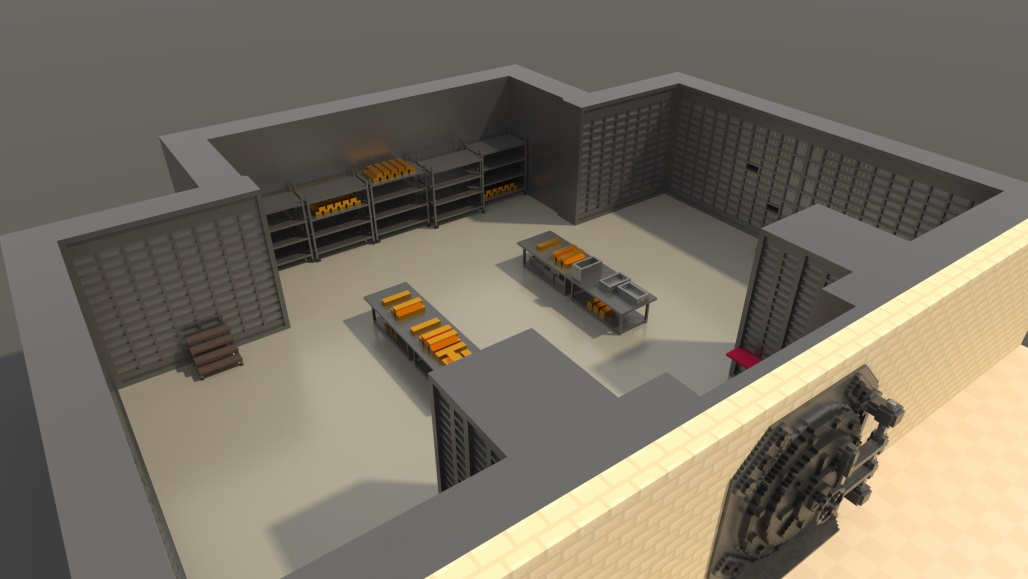
\includegraphics[width=\linewidth]{images/lookandfeel.jpg}
	\caption{Look and Feel}
\end{figure}

\chapter{Story and Setting}

\section{Story and Narrative}

Our setting is the Cinque National Bank (CNB), it is a prestigious and sophisticated bank frequented by the rich and known by thieves as a goldmine. Set in the near future, Cinque National Bank is notorious for their top of the line security and surveillance measures in addition to being loaded.  The bank is a complex building with a lot of hallways, rooms, and sections with state of the art defense and security mechanisms along with professional security drones. Although many thieves from all around the world have attempted to pull off heists, no one has been successful, so far. This time, however, four thieves plan to perform the biggest heist in history at Cinque National Bank, but little do they know, they are all there on the same night.

\subsection{Game Progression Summary}

Four thieves spawn at random at one of the four points of entry. In the first stage, their objective is to infiltrate the bank by getting past quicktime events to bypass traps and hazards. Secondly, they must now move through the bank to not get spotted by other players or security drones. 
Their next objective is to get to the vault and obtain as much gold as possible and more then the next player to win. After they need to obtain as much gold as possible from the bank, they have to escape through the bank from a randomly chosen escape point in the bank before the lockdown timer expires and they get stuck in the bank.

\section{Cut Scenes}
\subsection{(Introduction)}

All four characters are introduced to the player through a slanted comic book style to demonstrate to the player exposition of how the four thieves got to the bank (See concept below). This cutscene is triggered after the players have all selected their characters and enter the game.

\subsubsection{Description}

EXT. Outside of Bank -- NIGHT
\begin{itemize}
    \item Four characters are seen on the left side of the screen on one of the slanted comic book-like panels. 
    \item First panel is of the one of the four characters running/sneaking to the bank.
    \item Second panel is one of the four characters staring up at the bank in awe.
\end{itemize}
INT. Inside of Bank -- NIGHT
\begin{itemize}
    \item Third panel is one of the four characters breaking/sneaking into the bank.
    \item Last panel is one of the four character gesturing that they are ready to rob the bank.
\end{itemize}

\subsubsection{Storyboard}
%%TODO: (Insert Later)

\subsection{Victory Screen}
%%TODO: (Insert Later)

\section{Game World}

\subsection{General Look and Feel of the World}

\subsubsection{Ground Floor}

The ground floor will contain, office spaces, board/conference rooms, teller stations, restrooms, information booths used by the employees of the CNB.

The environment will remain clean and modern with simple geometric shapes i.e. chairs, tables, ATM’s and etc that are found throughout the bank.

\subsubsection{Basement}
%%TODO: (TBC)
The basement contains the vault.

\chapter{Characters}

\section{Marshal``King''}

\begin{figure}[H]
    \centering
    \includegraphics[width=.5\linewidth]{images/TheBig.jpg}
    \caption{Marshal ``King''}
\end{figure}

\subsection{Back Story}

King is a gang leader who comes from a neighborhood on the outskirts of a large city. In recent times, the neighborhood had fallen into financial troubles, and the residents who live there started stealing from each other to get by. Tired of having people trying to steal his stuff, King went all-in on his criminal career and set out for the biggest and richest banks in the world with the intention of sending the money back home to put his neighborhood back on top. Despite his intimidating appearance, King is a surprisingly calm and quiet person.

\subsection{Personality}

King is a good hearted man that has the soft spot for his community. His compassion to take care of his community is what motivates him to result to dangerous and criminal activity to do what is best for them.

\subsection{Physical Characteristics}

Marshal is a male, athletically built, African American, brown eyes, black hair, primarily long sleeves (top color variations for how many players choose King) dark bottoms and heavy boots/shoes.

\subsection{Animations}

Marshal “King” menu selection animation consists of him crossing his arm confidently and having a little smirk, showing the player his confidence and strength.

\subsection{Special Abilities}

Because of Marshal’s athletic ability, he has has one extra health stack which allows him to take more damage (stuns) from other players and/or security drones.

\subsection{Statistics}

\begin{itemize}
    \item Slower (2/4)
    \item Health (5/4)
    \item Lower Dexterity (2/4)
\end{itemize}

\begin{figure}[H]
    \centering
    \includegraphics[width=.5\linewidth]{images/kingui_sarah.jpg}
    \caption{}
\end{figure}

\section{Anna ``Jailbird''}
\begin{figure}[H]
    \centering
    \includegraphics[width=.5\linewidth]{images/TheJailbird.jpg}
    \caption{Anna ``Jailbird''}
\end{figure}

\subsection{Back Story}

Jailbird is an average thief with a not-so-average amount of enthusiasm. Stealing things is her passion, and she never gives up the opportunity for a good old-fashioned heist. Her happy-go-lucky nature has managed to get her caught on multiple occasions; but no matter how well the authorities try to keep her contained, Jailbird always manages to find a way to escape and jump right back into another crime spree.

\subsection{Personality}

Jailbird is eccentric, curious and mischievous .With her only motivation to steal and escape when captured.

\subsection{Physical Characteristics}

Ana “Jailbird” menu selection animation consists of her jumping and raising her arms high with excitement.

\subsection{Animations}

Ana “Jailbird” menu selection animation consists of her jumping and raising her arms high with excitement.

\subsection{Special Abilities}

Because of Ana’s criminal background, police are always in pursuit of her, building her stamina to being able to run faster and longer.

\subsection{Statistics}

\begin{itemize}
    \item Health Stack (4/4)
    \item Fastest Movement (5/4)
    \item Dexterity (3/4)
\end{itemize}

\begin{figure}[H]
    \centering
    
\includegraphics[width=.5\linewidth]{images/jailbirdui_sarah.jpg}
    \caption{}
\end{figure}

\section{Olivia ``Shadow''}

\begin{figure}[H]
    \centering
    \includegraphics[width=.5\linewidth]{images/TheShadow.jpg}
    \caption{Olivia ``Shadow''}
\end{figure}

\subsection{Back Story}

Shadow is a spy-for-hire with the promise of always getting the job done. Many mafia and organized crime groups across the world seek her out for whenever they’re in need of a good thief getting in and out without getting noticed. Money. Classified info. Prototype technology. You name it, she can steal it. Due to her perfect track record, Shadow has a cocky side to her. She often sees herself as unstoppable and has a tendency to taunt and charm her rival thieves.

\subsection{Personality}

Shadow is cool, adept and charming. She is able to find her way out of every sticky situation and break every problem.

\subsection{Physical Characteristics}

Olivia is a female, slender built, middle eastern ancestry, brown eyes, black hair, full body catsuit (top color variations for how many players choose King) and knee high black boots.

\subsection{Animations}

Olivia “Shadow” menu selection animation consists of her moving her hand with slight to reveal a jewel in her hand and the other on her hip.

\subsection{Special Abilities}

Because of her long history of being a spy-for-hire, she has required a real knack for hacking and breaking into the toughest of locks.

\subsection{Statistics}

\begin{itemize}
    \item Health (4/4)
    \item Speed (4/5)
    \item Dexterity (5/4)
\end{itemize}

\begin{figure}[H]
    \centering
    
\includegraphics[width=.5\linewidth]{images/shadowui_sarah.jpg}
    \caption{}
\end{figure}

\section{Rocco ``Racoon''}

\begin{figure}[H]
    \centering
    \includegraphics[width=.5\linewidth]{images/TheRaccoon.jpg}
    \caption{Rocco ``Racoon''}
\end{figure}

\subsection{Back Story}

Raccoon is a kleptomaniac who has an obsession with anything and everything shiny. He was originally a scavenger who would scour around junk piles and scrap yards for anything that seemed valuable. Soon enough he looked to bigger and better ambitions of stealing jewels and gold. His costume resembles that of a raccoon, hence his name, and his small build makes him surprisingly nimble and hard to catch than most other thieves.

\subsection{Personality}

From a young age, Rocco, a slight maniac just can’t keep his hands off anything that is remotely shiny or expensive. His body movements are sporadic and jerky due to his suspicious mentality that someone might want to take this ``shiny things''.

\subsection{Physical Characteristics}

Rocco is a male, medium built, Caucasian, blue eyes, tattered clothing, hair is disordered with two bunches are pointed up that resembles ears and wears a mask.

\subsection{Animations}

Rocco ``Racoon'' menu selection animation consists of him rubbing his hand together to portray that he is ready to take the big score.

\subsection{Special Abilities}

Because of his long history of stealing, Rocco has the ability to obtain loot faster than most thieves and has a longer range to grab pick ups.

\subsection{Statistics}
\begin{itemize}
    \item Health (4/4)
    \item Speed (4/4)
    \item Dexterity (4/4)
\end{itemize}

\begin{figure}
    \centering
    \includegraphics[width=.5\linewidth]{images/raccoonui_sarah.jpg}
    \caption{}
\end{figure}

\section{A.S.I.A (NPC)}

\begin{figure}[H]
    \centering
    \includegraphics[width=.3\linewidth]{images/drone_face.jpg}
    \includegraphics[width=.3\linewidth]{images/drone_face.jpg}
    \caption{A.S.I.A}
\end{figure}

\subsection{Back Story}

A.S.I.A stands for Artificial Security Intelligence Administrator, and is the name of the AI developed by the CNB Security Technologies team to control the bank’s security system. She is a highly advanced AI bot that controls the drones and traps 24 hours per day. A.S.I.A will be responsive to the player’s actions and will dish out trash talk whenever the fail.

\subsection{Personality}

A.S.I.A was developed to be a sassy, pretentious, and cocky character to destroy any potential intruder’s confidence and lead them to more errors. She looks down upon any intruder, and believes her security mechanisms are impenetrable.


\chapter{Gameplay and Mechanics}

\section{Game Progression}
Game Progression split into 3 parts

\subsection{Infiltration}
\begin{itemize}
    \item Infiltration stage implies that the players must sneak in to the bank and make their way towards the basement.
    \item Infiltration stage will require players to be more stealthy
    \item Players can engage in combat
    \item Players will familiarize themselves with the environment and its challenges in this stage
\end{itemize}
\subsection{Scavenging}
\begin{itemize}
    \item This stage of the game blends between the other two stages
    \item Players will collect weapons and traps
    \item Players will set traps across the map for other players
    \item They will explore rooms and hallways for loot 
\end{itemize}
\subsection{Lockdown}
\begin{itemize}
    \item This stage will be the most chaotic stage of the game
    \item As soon as a player accesses the vault, a lockdown timer initiates
    \item In this stage, players will be rushing and battling to gather as much gold as possible and try to escape the bank before lockdown.
    \item Only one exit will be available
    \item More traps and hazards will spawn
    \item Drones will be more aggressive
\end{itemize}

\begin{figure}[H]
    \centering
    \includegraphics[width=\linewidth]{images/progPic.jpg}
    \caption{Game Progression}
\end{figure}

\section{Objectives}
\subsection{Main Objectives}
\begin{itemize}
    \item Achieve the highest score possible by collecting gold from the vault
    \item Escape before lockdown
\end{itemize}

\begin{figure}[H]
    \centering
    \includegraphics[width=\linewidth]{images/insidebank.jpg}
    \caption{}
\end{figure}

\subsection{Secondary Objectives}
\begin{itemize}
    \item Dodge and disable traps and hazards
    \item Collect weapons and traps
    \item Use weapons to engage in combat with players and/or drones
    \item Set up traps
    \item Unlock doors
\end{itemize}

\section{Challenges}    
\subsection{Level Layout}
\begin{itemize}
    \item Levels are not going to be straightforward paths towards the vault
    \item Levels will contain multiple paths, each with their own pros and cons
    \item Level of difficulty and frequency of pickups will vary area to area
    \item Hazards will already be set in the map at the beginning of the game
    \begin{itemize}
        \item Laser Tripwire: will inform enemy drones to the players position and send them to the player's area
        \item Electric Field: Damages (1DMG) and slows players
        \item Lethal Lasers: Damages players (2 DMG)
    \end{itemize}
    \item Hazards will be strategically set at areas of importance
    \item Some hazards can be disabled temporarily through a quick-time event
    \begin{itemize}
        \item If quick-time event is successful, trap is disabled for a short amount of time
        \item If quick-time event is failed, trap is triggered
    \end{itemize}
\end{itemize}

\subsection{Security Drones}
\begin{itemize}
    \item Drones are the primary enemy for the players
    \item They patrol the bank, and will detect players in their vision radius
    \item Drones will attack the player if a player is detected
    \item Drones will be equipped with either of the following weapons
    \begin{itemize}
        \item Stun Gun: ranged weapon that charges up before firing (dodge-able)
        \item Electric Field: AoE weapon that drones can deploy for short bursts, it deploys an electric field under them that will damage players that step in it. Drones will be faster and chase players around
    \end{itemize}
    \item Drones will drop gold when they are damaged or stunned
    \item Drones will need to gain 3 stacks to be stunned.
\end{itemize}

\subsection{Combat}
\begin{itemize}
    \item Players can engage in combat with other players and/or drones.
    \item Players will have a default melee weapon unique to each character.
    \item Players will also have 2 weapons that are available as pickups:
    \begin{itemize}
        \item Stun gun: Semi-auto weapon that shoots in a certain direction and damages enemies.
        \item Electric Baton: Melee weapon that does high damage, and applies a short stun.
    \end{itemize}
    \item Weapons will have limited uses (ammo).
    \item Players will have 2 traps that are available as pickups:
    \begin{itemize}
        \item Lethal Lasers: will damage players if they step into it.
        \item Electric Field: AoE field, will slow and damage players over time.
    \end{itemize}
\end{itemize}


\section{Mechanics}
\subsection{Physics}
\subsection{Movement}

The player can move in all directions along the xz plane, and can also use a dash.

\subsection{Scoring System}
\begin{itemize}
    \item Score will be calculated according to how much gold is collected
    \item Player with the highest score (that manages to escape) will win
    \item 1 Gold = 1 Score
    \item When players get damaged/stunned and drop gold, they will lose score
    \item Each drone will drop X amount of gold only
\end{itemize}

\subsection{Health System}
\begin{itemize}
    \item Players and drones will share the same health system
    \item Health system will be a 4-hit system
    \begin{itemize}
        \item 1 Damage point will reduce a Health Stack on the player/drones
        \item Health stack will regain after 20 seconds for the first stack and 5 seconds for the following stacks, if player/drone is not damaged
        \item If player/drone manages to get max stacks, they will be stunned for 5 secs
        \item If player is attacked while stunned, or up to 3 seconds after a stun, no stacks will be applied
    \end{itemize}
    \item Player/drones will drop X amount of gold when damaged
    \item Player/drones will drop Y amount of gold when stunned
\end{itemize}

\subsection{Pick Up System}
\begin{itemize}
    \item Pickups are available in designated areas in the map
    \item Pickups respawn every 45 secs
    \item There is a minimum and maximum number of pickups available at all times
\end{itemize}

\subsection{Interactions}
\begin{itemize}
    \item Players can interact with pickups to add to their inventory
    \item Players can also interact with traps and locked doors to disable/unlock them
    \begin{itemize}
        \item Players will be presented with either quicktime event challenge
        \begin{itemize}
            \item Players will have to press space at the right time to stop the arrows in the right area to disable traps. If failed, trap will activate
            \item Players will have to quickly tap buttons in the right order to unlock doors. If failed, nearby drones will gain gold, if failed, player will lose gold.
        \end{itemize}
    \end{itemize}
    \item Players can interact with gold piles in the vault and will be presented with quicktime challenges. If successful, player will gain bonus gold, if failed, player will lose gold.
\end{itemize}

\section{Combat}

\begin{itemize}
    \item Players will be able to engage in combat with:
    \begin{itemize}
        \item Other Player Characters
        \item Drones
    \end{itemize}
    \item Players will have a basic melee attack that does no damage but pushes players/drones away.
    \item Weapons will also push away enemies.
    \item Player \emph{Weapons} that will be available as pickups across the map:
\end{itemize}

\subsection{Player Weapons}


\begin{itemize}
    \item \textbf{Stun Gun}:
    \begin{itemize}
        \item Shoots a projectile in a straight line.
        \item Projectile will do 1 DMG when enemy is hit 
        \item Projectile will disappear upon impact
        \item Player gets 5 shots (ammo) per Stun Gun pickup
        \item After 5 shots, Stun Gun will disappear from inventory
    \end{itemize}
\end{itemize}

\begin{figure}[H]
    \centering
    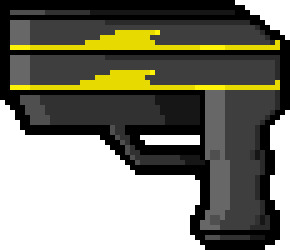
\includegraphics[width=.2\linewidth]{images/zappy_gun.jpg}
    \caption{}
\end{figure}

\begin{itemize}
    \item \textbf{Electric Baton}
    \begin{itemize}
        \item Activatable weapon, does AoE DMG around character
        \item Does 1 DMG per hit
        \item Pushes enemies away
        \item Melee weapon that increases player movement speed by 30%
        \item Lasts for 8 secs (Active)
    \end{itemize}
\end{itemize}

\begin{figure}[H]
    \centering
    \includegraphics[width=.2\linewidth]{images/zappy_stick.jpg}
    \caption{}
\end{figure}
    
\subsection{Player Traps}

\begin{itemize}
    \item \textbf{Electric Field}:
    \begin{itemize}
        \item Pick up
        \item Can be deployed on any tile (if the tile has no traps already)
        \item AoE damage field
        \begin{itemize}
            \item Does 1 Damage/2secs
            \item Slows Players Movement Speed by 25\%
            \item Lasts for 2 Minutes if untriggered
            \item Lasts for 30 secs after triggered
        \end{itemize}
    \end{itemize}
    \item \textbf{Lethal Lasers}:
    \begin{itemize}
        \item Pick up
        \item Can be deployed on any tile (if the tile has no traps already)
        \item On-Contact damage
        \begin{itemize}
            \item Does 2 Damage/contact
            \item Lasts for 2 Minutes if untriggered.
            \item Disappear after trigger.
        \end{itemize}
    \end{itemize}
\end{itemize}

\subsection{Inventory System}

\begin{itemize}
    \item An inventory system will be in place for weapons and traps pickups
    \item Pickups will be available across the map 
    \begin{itemize}
        \item Players will need to be in range to pick up a weapon or trap
        \item A button prompt will appear when player in range
        \item Player can press button to pick up weapon/trap
    \end{itemize}
    \item Picking up a weapon that the player already has refreshes the ammo
    \item Picking up a trap that the player already has adds to the ammo (Max 4)
    \item Players presses button to cycle between items
\end{itemize}

\subsection{Inventory System}

\begin{itemize}
    \item An inventory system will be in place for weapons and traps pickups
    \item Pickups will be available across the map 
    \begin{itemize}
        \item Players will need to be in range to pick up a weapon or trap
        \item A button prompt will appear when player in range
        \item Player can press button to pick up weapon/trap
    \end{itemize}
    \item Picking up a weapon that the player already has refreshes the ammo
    \item Picking up a trap that the player already has adds to the ammo (Max 4)
    \item Players presses button to cycle between items    
\end{itemize}

\section{Screen Flow}
\subsection{Screen Flow Chart}

\begin{figure}[H]
    \centering
    \includegraphics[width=\linewidth]{images/screenFlow.jpg}
    \caption{Screen Flow Chart}
\end{figure}

\subsubsection{Main Menu Screen}

First Screen that the player has access to. Contains Start Game, Options, and Exit Game buttons.

\begin{figure}[H]
    \centering
    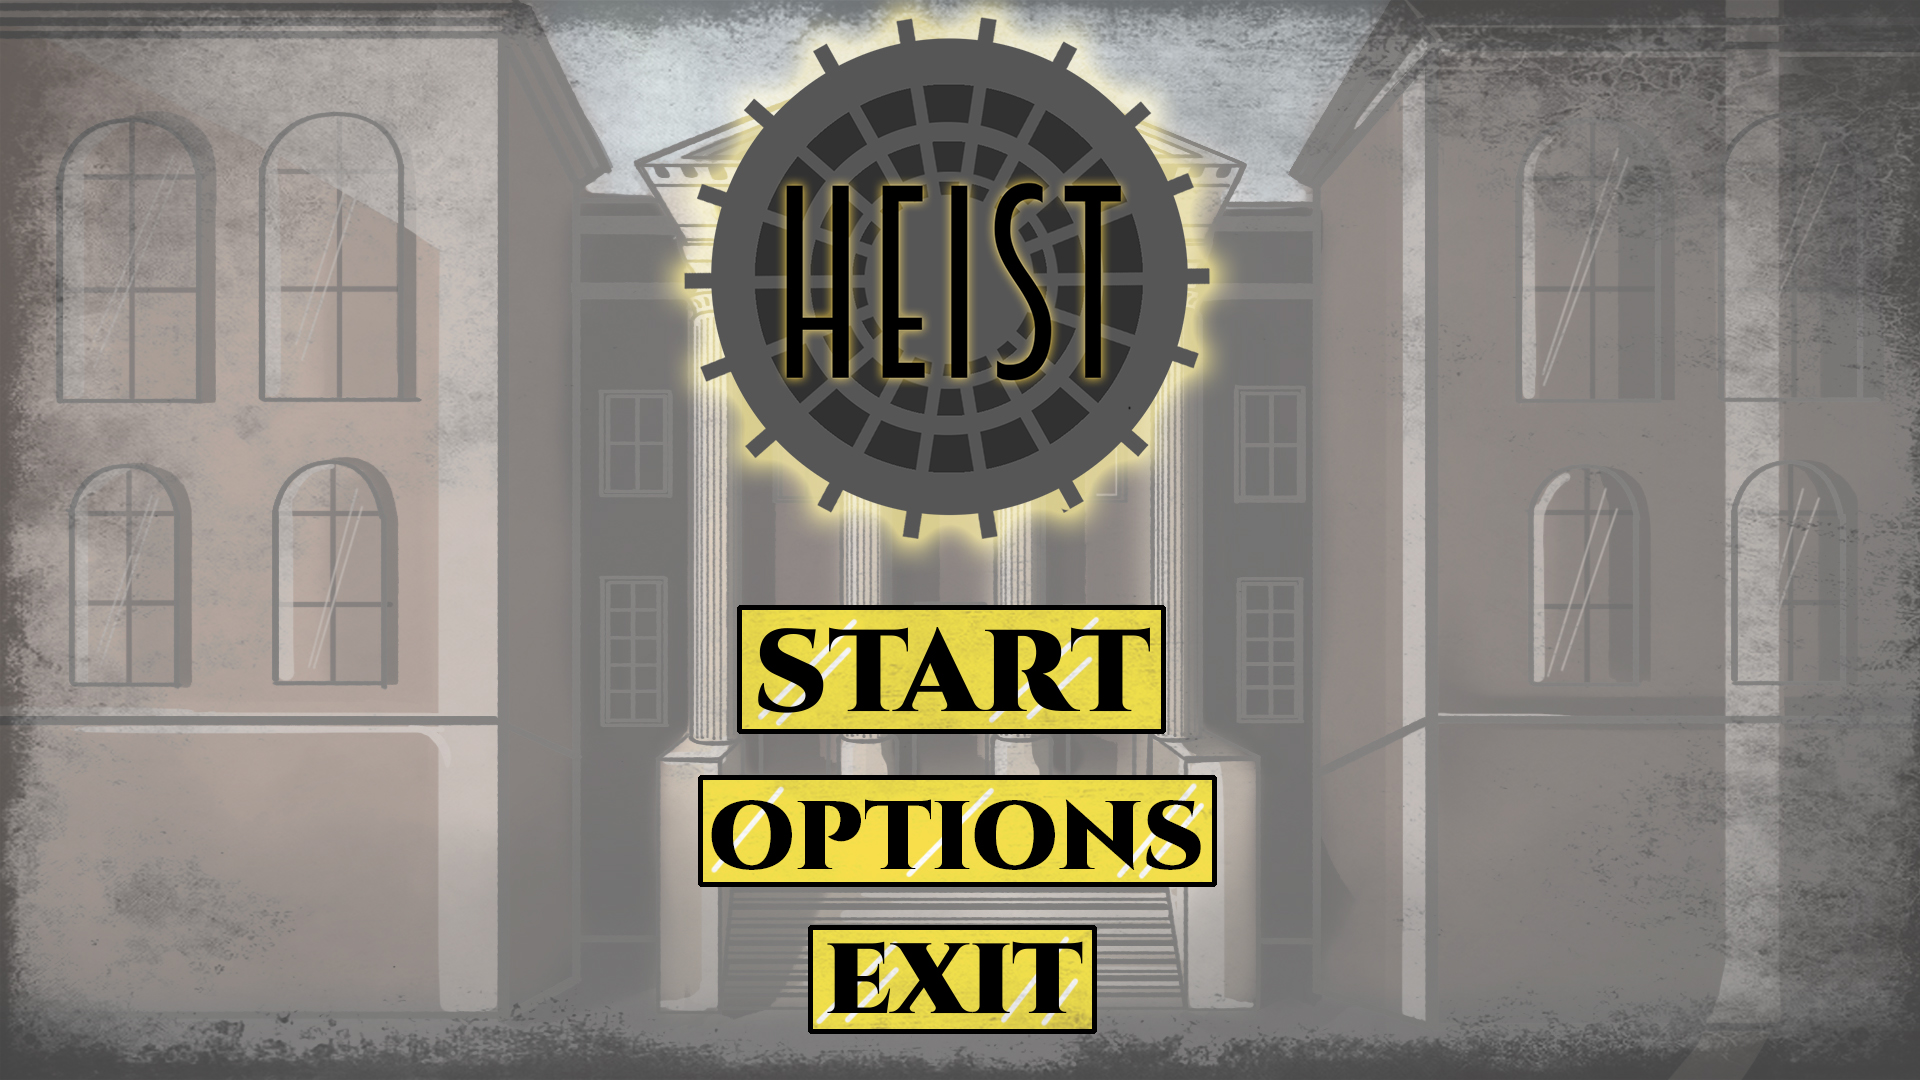
\includegraphics[width=\linewidth]{images/menu.jpg}
    \caption{}
\end{figure}

\subsection{Game Screen}

\begin{itemize}
    \item This screen starts after player selects Start Game, and includes multiple other screens.
    \begin{itemize}    
        \item \textbf{Character Selection}: In this menu, players select their characters before the match starts
        \item \textbf{Intro Cutscene}: This cutscene plays before the match starts, giving context for the game and explains the setting.
        \item \textbf{Play State}: This screen includes everything in the actual game, from UI to the Characters. It is the main screen the players are going to be on.
        \item \textbf{End Game Screen}: This screen shows the winner’s character splash art then all of the players ranked in order of score in front of the vault. This screen contains Main Menu and Exit Game buttons
    \end{itemize}
\end{itemize}

\subsection{Options Menu Screen}
\begin{itemize}
    \item This screen can be access through the \textbf{Main Menu} by selecting the \textbf{Options} button. It contains multiple other screens.
    \begin{itemize}
        \item \textbf{Controls}: This shows the controls for both controllers and keyboard
        \item \textbf{Audio/Video}: This allows the player to customize Audio and Video settings
        \item \textbf{Credits}: This shows the credits screen.    
    \end{itemize}
\end{itemize}

\chapter{Levels}

\section{Floor \#1}

\subsection{Synopsis}

The Ground Floor is the starting point for all characters. It contains the player spawn points. This floor has a lower number of pickups and obstacles than the Basement Floor. There are hazards and traps around, but very few in comparison to the lower level of the bank.

\subsection{Physical Description}

The map contains many shades of grey and dark colours such as azure blue and seaweed green. It’s viewed in a top-down, Isometric angle. The rooms present are offices, lobbies, meeting rooms, and bathrooms. They are all connected through a series of long hallways that will be filled with hazards and drones.

\subsection{Map}

\begin{figure}[H]
    \centering
    \includegraphics[width=.8\linewidth]{images/Ground.png}
    \caption{Ground Floor Map}
\end{figure}

\begin{figure}[H]
    \centering
    \includegraphics[width=.5\linewidth]{images/Legend.png}
    \caption{Legend}
\end{figure}

\subsubsection{Primary Path}

(Shown in Blue) The player spawns and makes their way directly down the stairs to the vault. This way is the fastest, but the players miss out on valuable pickups.

\subsubsection{Secondary Path}

(Shown in Magenta) The player spawns and looks around the bank for pickups. This way they gain an advantage against other players and drones, but it is not as fast as just going to the ground floor.

\begin{figure}[H]
    \centering
    \includegraphics[width=.8\linewidth]{images/GroundPathing.png}
    \caption{Player Pathing on Ground Floor}
\end{figure}

\subsection{Encounters}

The player will encounter various challenges. The drones will attempt to stun them, and other players will be trying to prevent them from making it to the vault. There will also be various types of hazards that will slow the player down. The multiple Drones follow the yellow paths in opposite directions.

\begin{figure}[H]
    \centering
    \includegraphics[width=.8\linewidth]{images/GroundDrone.png}
    \caption{Drone Pathing on Ground Floor}
\end{figure}

\subsection{Closing Material}

At the end of the game, the players will view a victory screen. The screen will show all four players as well as how much gold each player acquired. The players will be ranked in the order of how much gold they stole

\section{Floor \#2}

\subsection{Synopsis}

The basement floor is accessible through the staircases on the first floor. The basement contains a large amount of pickups and hazards - far more than the first floor. The vault is also located in the center of the basement. The players must go here to get the gold

\subsection{Physical Description}

The map contains many shades of grey and dark colours such as azure blue and seaweed green. It’s viewed in a top-down, Isometric angle. The rooms present are security rooms, more offices, storage rooms, and server rooms, in addition to the large gold vault.

\subsection{Map}

\begin{figure}[H]
    \centering
    \includegraphics[width=.8\linewidth]{images/Basement.png}
    \caption{Basement Floor Map}
\end{figure}

\subsubsection{Primary Path}

(Shown in Blue) The player gets down the stairs and immediately makes their way to the vault. This way is the fastest, but the players miss out on valuable pickups around the basement.

\subsubsection{Secondary Path}

(Shown in Magenta) The player gets down the stairs and looks around the basement for pickups. This way they gain an advantage against other players and drones, but it is not as fast as just going to the vault.


\begin{figure}[H]
    \centering
    \includegraphics[width=.8\linewidth]{images/BasementPathing.png}
    \caption{Player Paths on Basement}
\end{figure}

\subsection{Encounters}

The player will encounter various challenges. The drones will attempt to stun them, and other players will be trying to prevent them from making it to the vault. There will also be various types of hazards that will slow the player down. There will be far more hazards and drones in the basement. The multiple Drones follow the yellow path in opposite directions.


\begin{figure}[H]
    \centering
    \includegraphics[width=.8\linewidth]{images/BasementDrone.png}
    \caption{Drone Pathing on Basement}
\end{figure}

\chapter{User Interface}

\section{UI Layout}

As seen in Figure~\ref{fig:uilayout}, the UI elements will appear on the corner of each respective player's screen. The elements shown in the UI are going to be:

\begin{itemize}
\item \textbf{Player Health}: Health is represented using the red bars
\item \textbf{Gold Score}: Score is represented above the health using numbers
\item \textbf{Character Profile}: A picture of the selected character
\item \textbf{Active Item}: An icon of the selected weapon/trap 
    \begin{itemize}
        \item This will disappear if player doesn’t switch/use weapons/traps for 10 secs
    \end{itemize}
\end{itemize}

\begin{figure}[H]
	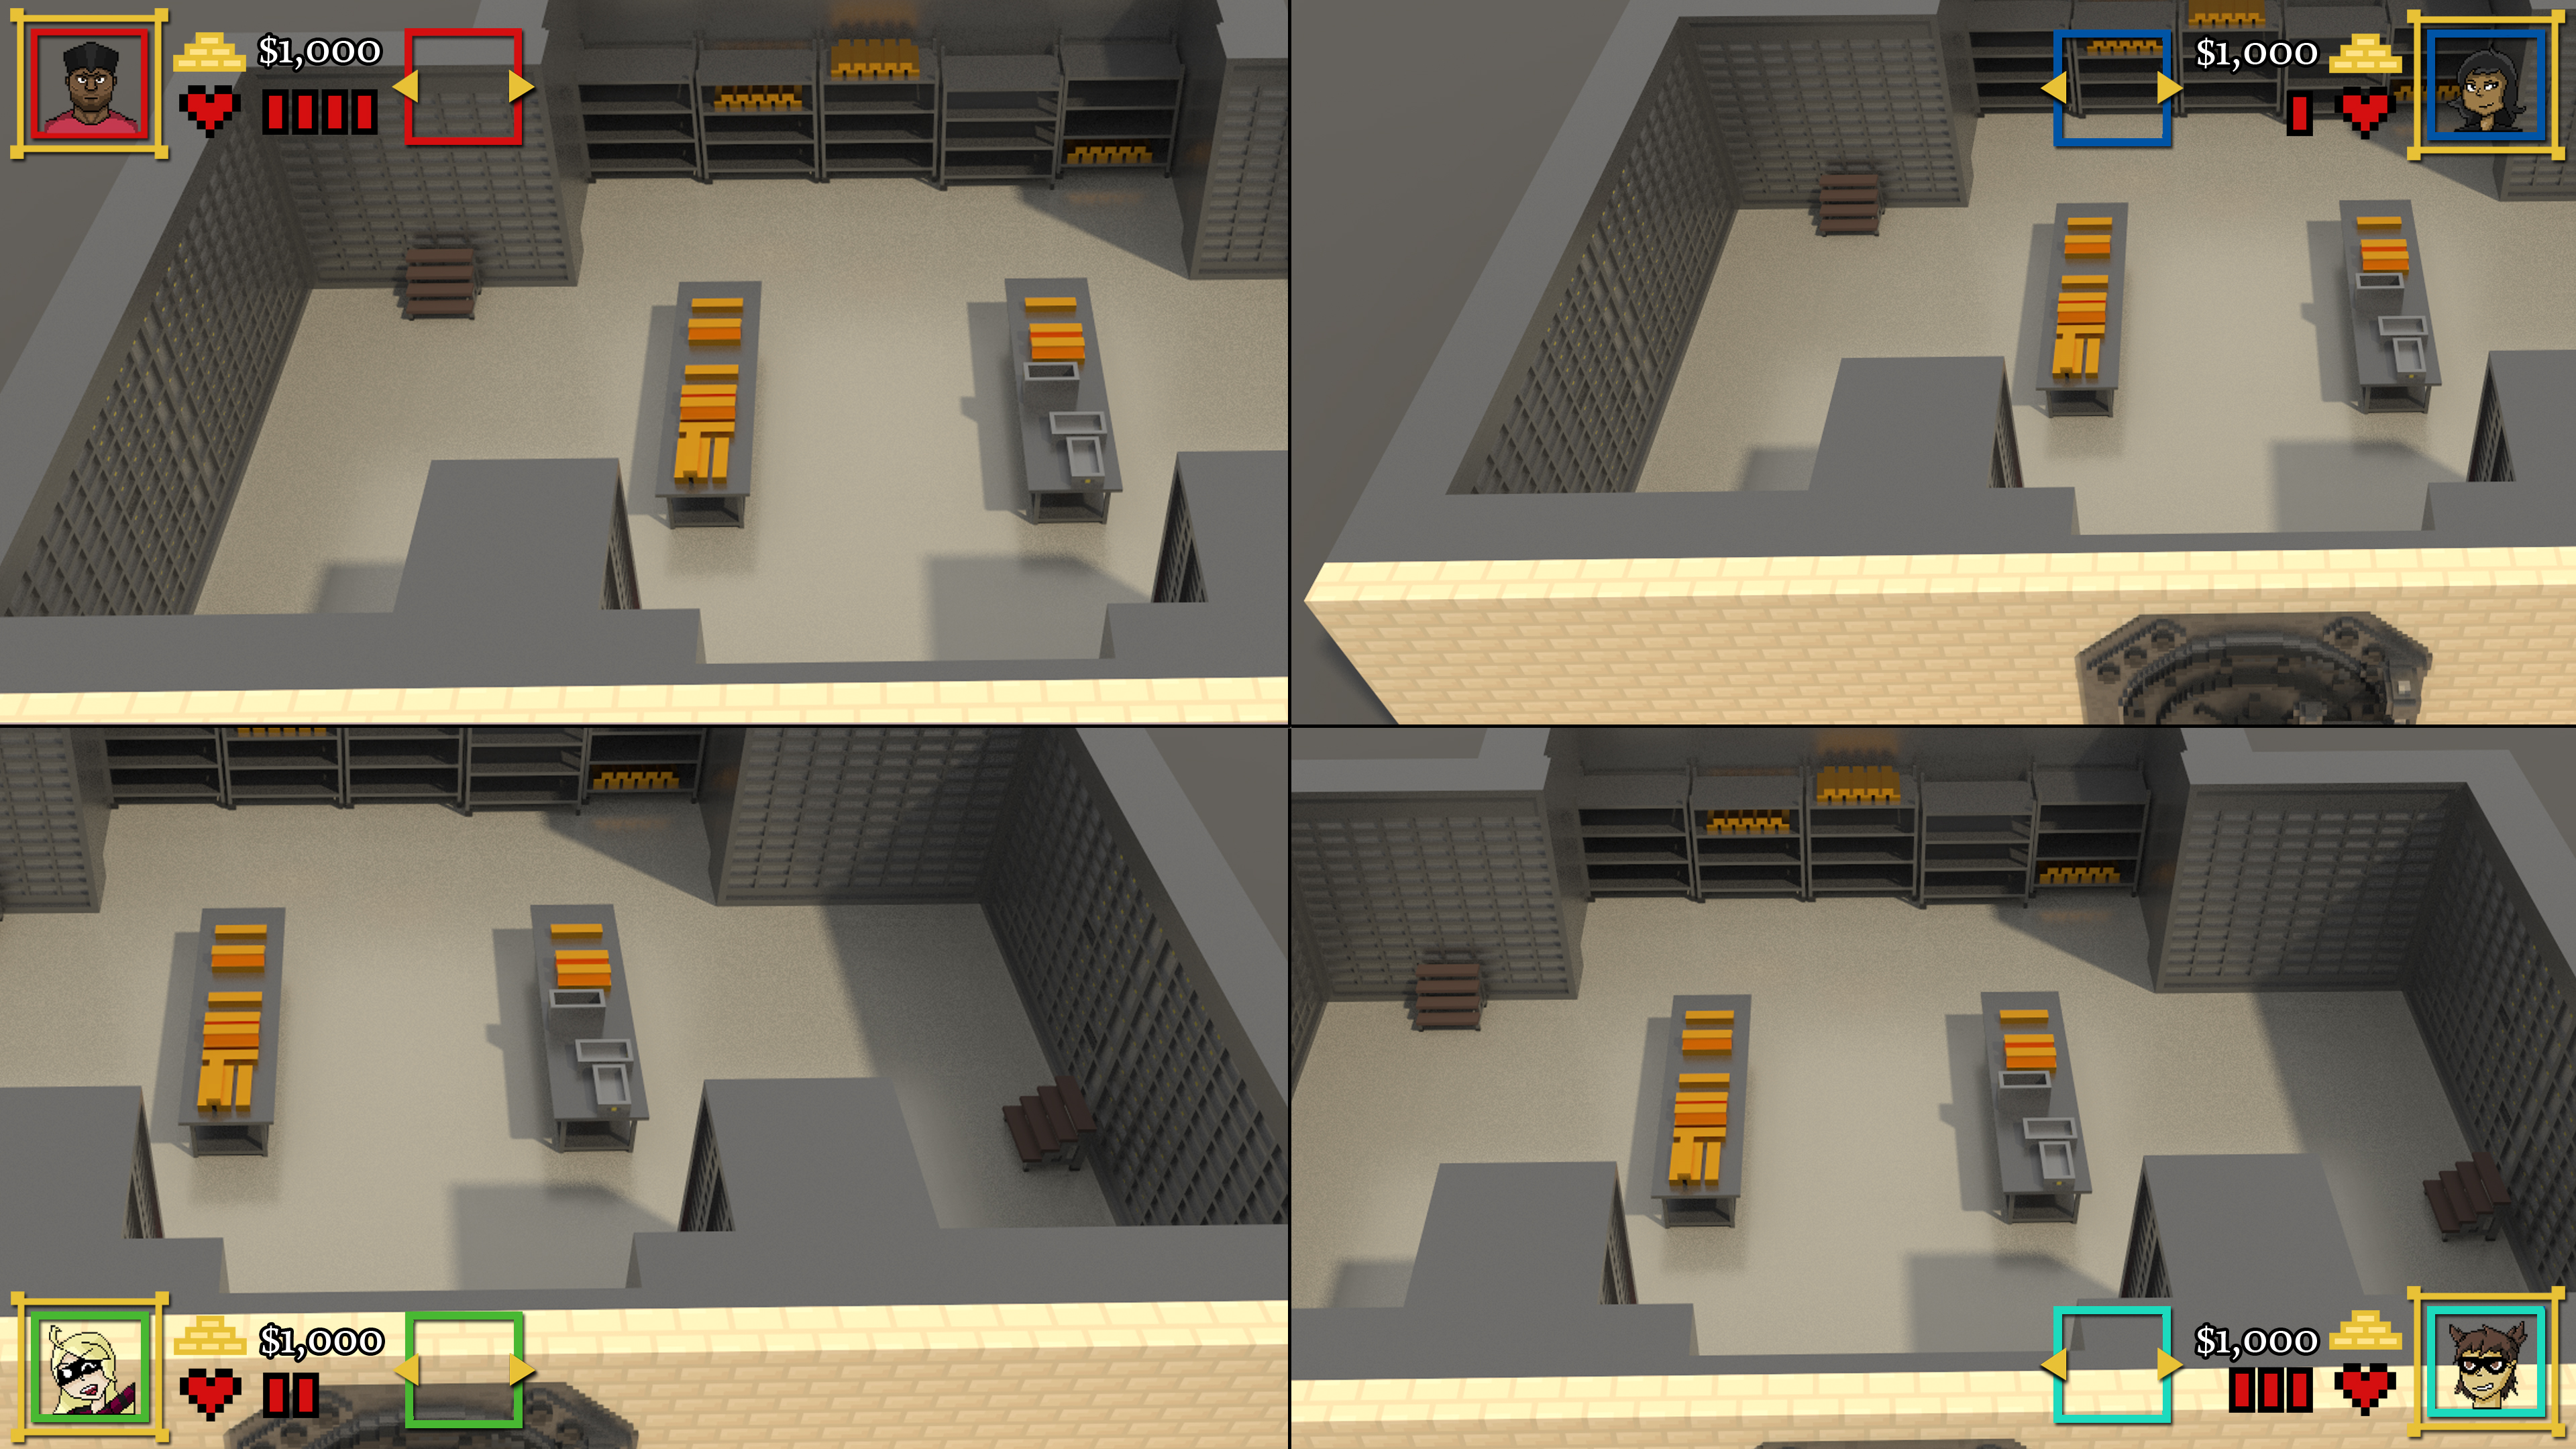
\includegraphics[width=\linewidth]{images/uiLayout.jpg}
    \caption{UI Layout}
\label{fig:uilayout}
\end{figure}

\section{Menus}

The only in-game menu available is the pause menu. It will include 2 buttons:

\begin{itemize}
    \item \textbf{Resume Game}: Exits pause screen and continues game.
    \item \textbf{Exit Game}: Exits game
    \begin{itemize}
        \item If a player exits a game, their controller will be disconnected. If controller is connected again, player can jump back in where they last stopped 
    \end{itemize}
\end{itemize}

Gameplay will only pause if two or more players bring up the pause menu


\section{Camera}

%%TODO: Add this

\section{Control Scheme}

Players could use either Keyboard/Mouse or a controller to play Heist.

\begin{figure}[H]
	\includegraphics[width=\linewidth]{images/keyboardlayout.jpg}
    \caption{Keyboard Control Layout}
\end{figure}

\begin{figure}[H]
	\includegraphics[width=\linewidth]{images/controllerlayout.jpg}
    \caption{Controller Control Layout}
\end{figure}

\section{Audio}

\begin{itemize}
    \item Audio prompts will aid the players comprehension on when key events are happening in game
\end{itemize}

\section{Music}

\begin{itemize}
    \item Three general themes will be present, and be active once a certain stage in the game has passed:
    \begin{itemize}
        \item Infiltration Phase
        \item Scavenging Phase
        \item Lockdown Phase
    \end{itemize}
    \item Additionally, different “jingles” will play depending on the outcome of the match for the player:
    \begin{itemize}
        \item Victory Jingle
        \item Defeat Jingle
    \end{itemize}
\end{itemize}

\section{Sound Effects}

\begin{itemize}
    \item Sound effects will play depending on the situation:
    \begin{itemize}
        \item Picking up an object
        \item Placing a trap
        \item Succeed/fail a quicktime event
        \item Taking damage
        \item Opening a door
        \item Collecting/dropping gold
        \item Attacking with weapons
        \item Drones
        \item Activating a trap
        \item Lockdown Siren
    \end{itemize}
\end{itemize}

\section{Help System}

\begin{itemize}
    \item Button prompts will appear when player is:
    \begin{itemize}
        \item Close to a pickup
        \item Close to an unlockable door
        \item Close to a gold pile in the vault
    \end{itemize}
    \item Controls will be shown in the beginning of each match after the cutscene.
\end{itemize}

\chapter{Artificial Intelligence}
\section{Enemy AI}

Drones

\begin{itemize}
    \item Patrols a set path until alerted and returns to the path once threat level returns to zero
    \item If it is alerted by a sound, the threat level becomes one and attempts to find the source of the sound
    \begin{itemize}
        \item It will go to the place the sound originated at, and once there begin a patrol of the area. Once patrol is complete and it doesn’t see anything, it’s threat level returns to zero and resumes it initial patrol.
    \end{itemize}
    \item If it sees a player, its threat level goes to two and attempts to follow and stun the player.
    \begin{itemize}
        \item If it loses site of the player for 5 secs, the threat level becomes one, and it will begin to patrol the area.
        \item If the drone successfully stuns the player, it will pick up a portion of gold (if dropped) and return it to the vault. Once the gold has been returned, the threat level returns to zero and the initial patrol is resumed.
    \end{itemize}
    \item If the drone, while following or patrolling an area, moves beyond a set distance from its original patrol, it will disengage, set its threat level to zero and return to its original patrol.
    \item Once the lockdown has been activated, the drones will begin threat level three, where their patrol distance is increased and their speed is increased.    
\end{itemize}

\section{Pathfinding}

Uses the default Unity Navmesh Agent, setting the focused player’s as the Drone’s target. When returning to the vault all players are swapped to obstacles with width wide enough to block the hallway, so the drone’s pathfinding will avoid them.

\section{Drone Finite State Machine}

\begin{figure}[h!]
	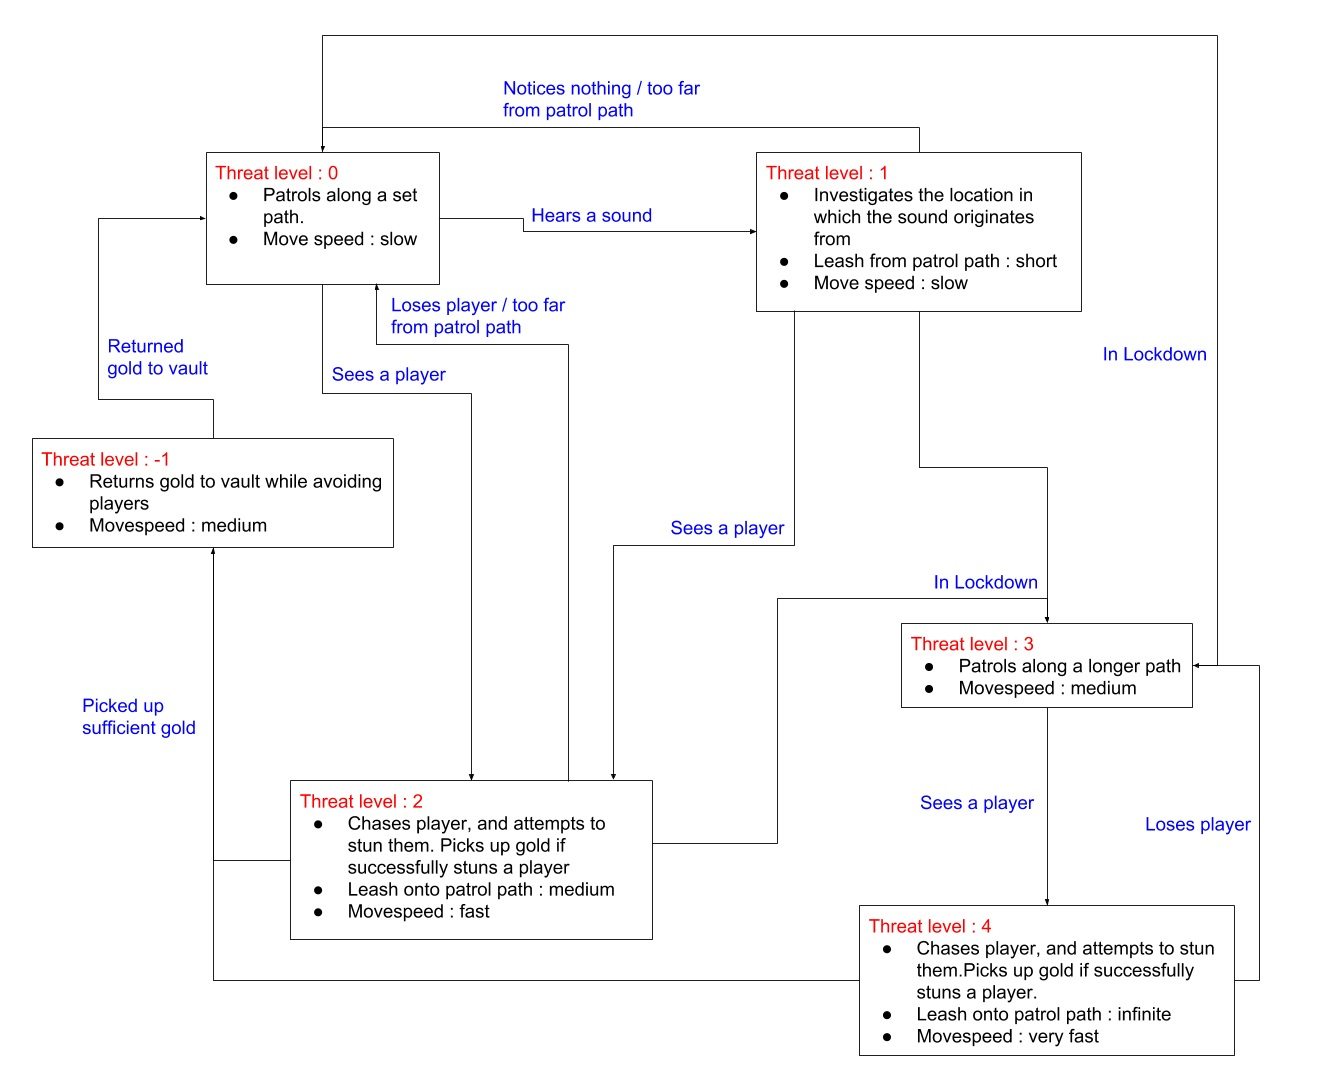
\includegraphics[width=\linewidth]{images/fsm-ai.jpg}
	\caption{Drone FSM}
\end{figure}

\chapter{Technical}

\section{Target Hardware}

Target hardware is as follows:

\begin{tabular}{|l|l|l|}
    \hline
     & Minimum & Recommended \\ \hline
     CPU & Pentium G4500 or Equivalent & Core i3-8500 or Equivalent \\ \hline
     GPU & AMD 7750 or Equivalent & AMD 260X or Equivalent \\ \hline
     RAM & 2 GB & 4 GB \\ \hline
     OS & Windows & Windows \\
    \hline
\end{tabular}

\section{Game Engine}

The game engine will be Unity 2018.4 LTS once it has been released. Pre-production work will be done in the most up to date version of Unity.

\section{Scripting Language}

All scripts are written in C\# following the guidelines that are outlined on Microsoft C\# Coding Conventions

\chapter{Game Art}

\section{Concept Art}

\begin{figure}[H]
	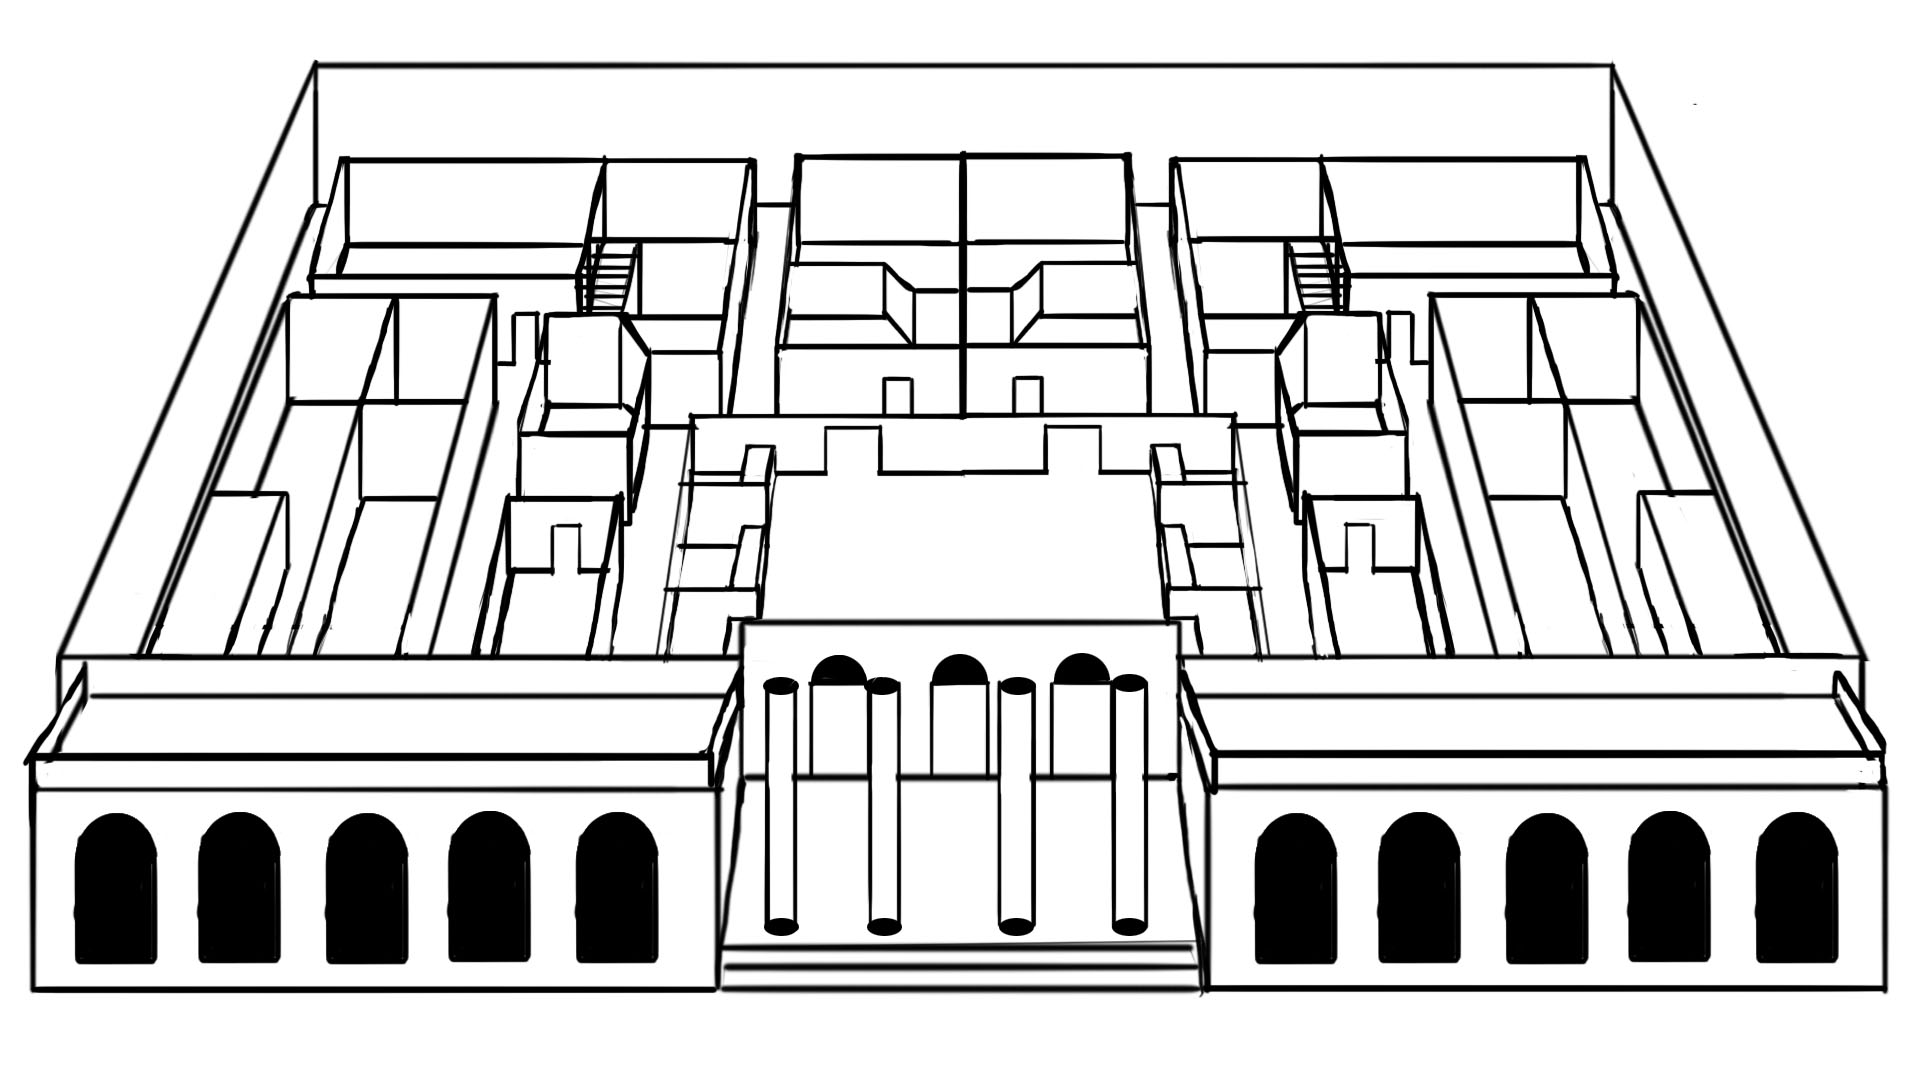
\includegraphics[width=\linewidth]{images/bankconcept.jpg}
    \caption{Early layout showing perspective}
\end{figure}

\begin{figure}[H]
    \centering
    
\includegraphics[width=.4\linewidth]{images/floortile.jpg}
    \includegraphics[width=.4\linewidth]{images/painting.jpg}
    \caption{Assets for Bank interior}
\end{figure}

\begin{figure}[H]
	
\includegraphics[width=\linewidth]{images/options.jpg}
    \caption{Logo concepts}
\end{figure}

\begin{figure}[H]
	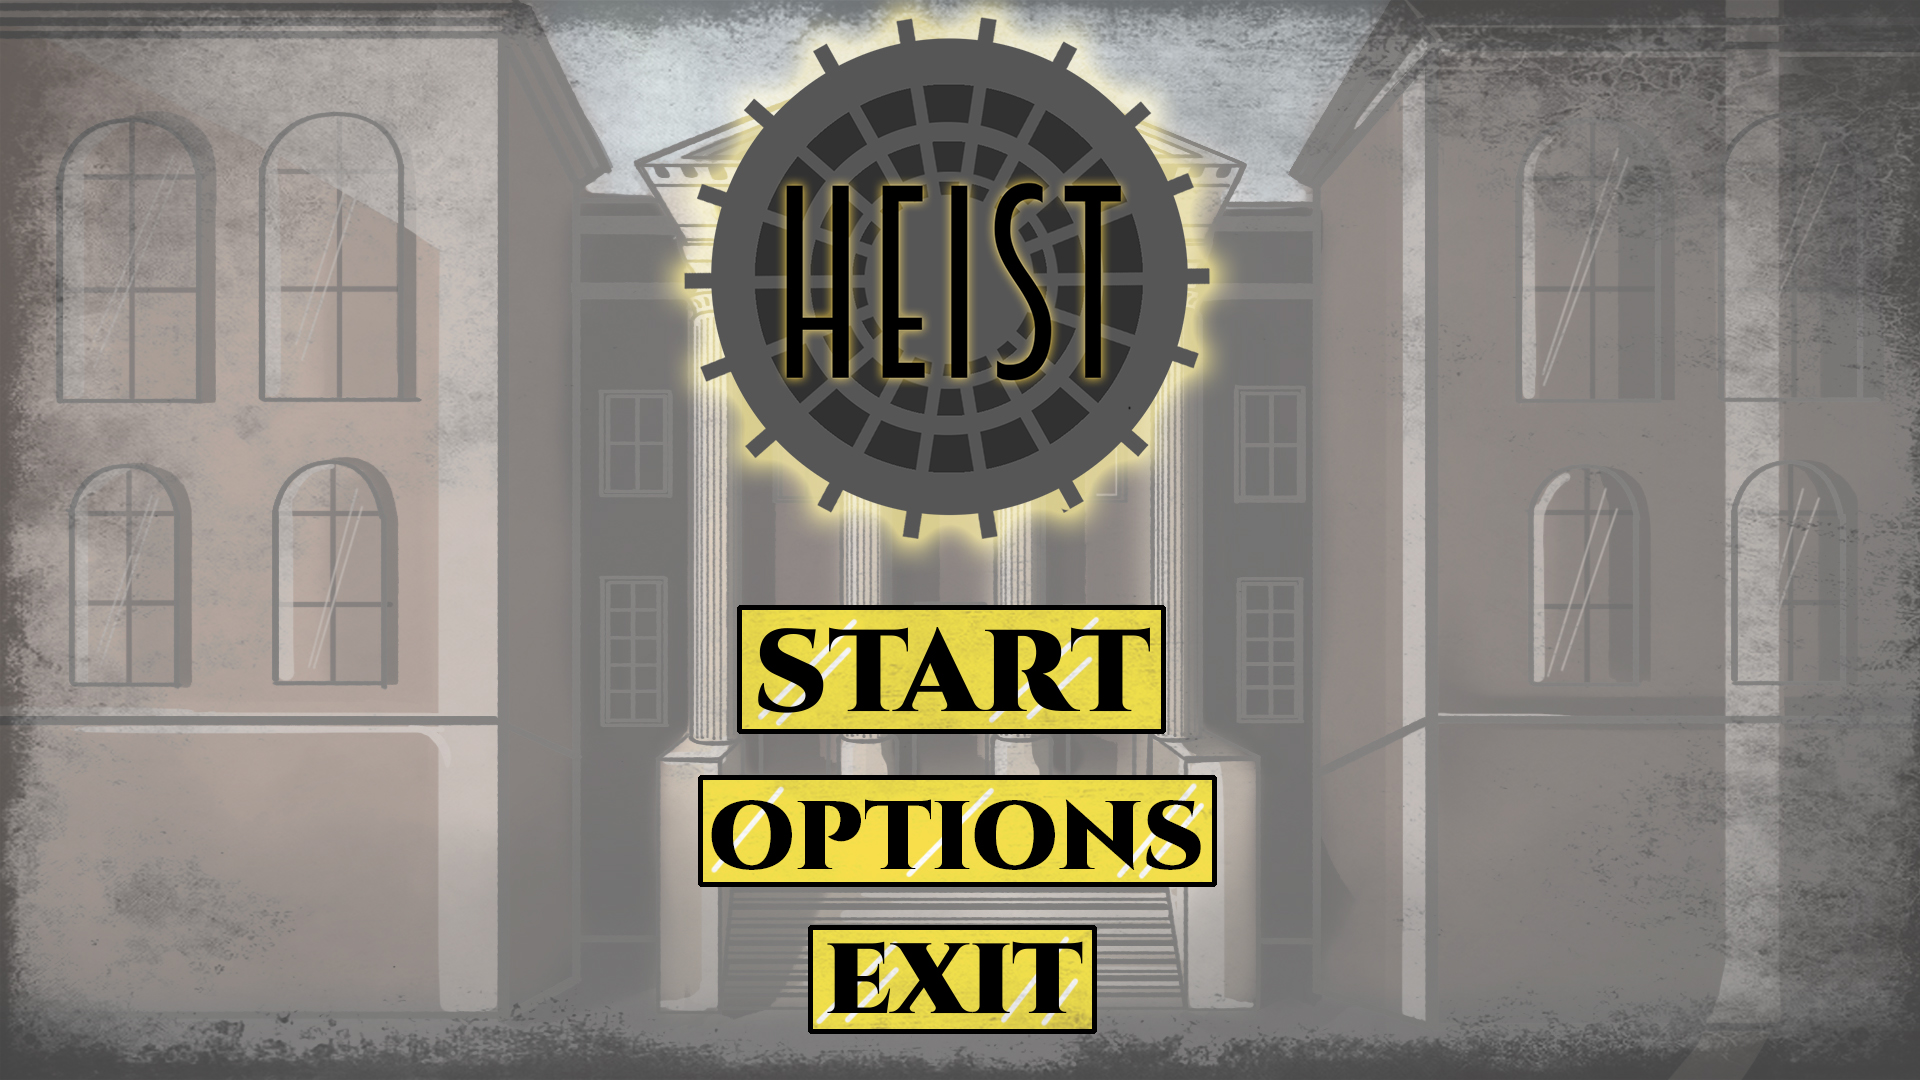
\includegraphics[width=\linewidth]{images/menu.jpg}
    \caption{Main Menu}
\end{figure}

\begin{figure}[H]
	\includegraphics[width=\linewidth]{images/ingameui.jpg}
    \caption{Early UI Concept}
\end{figure}

\begin{figure}[H]
	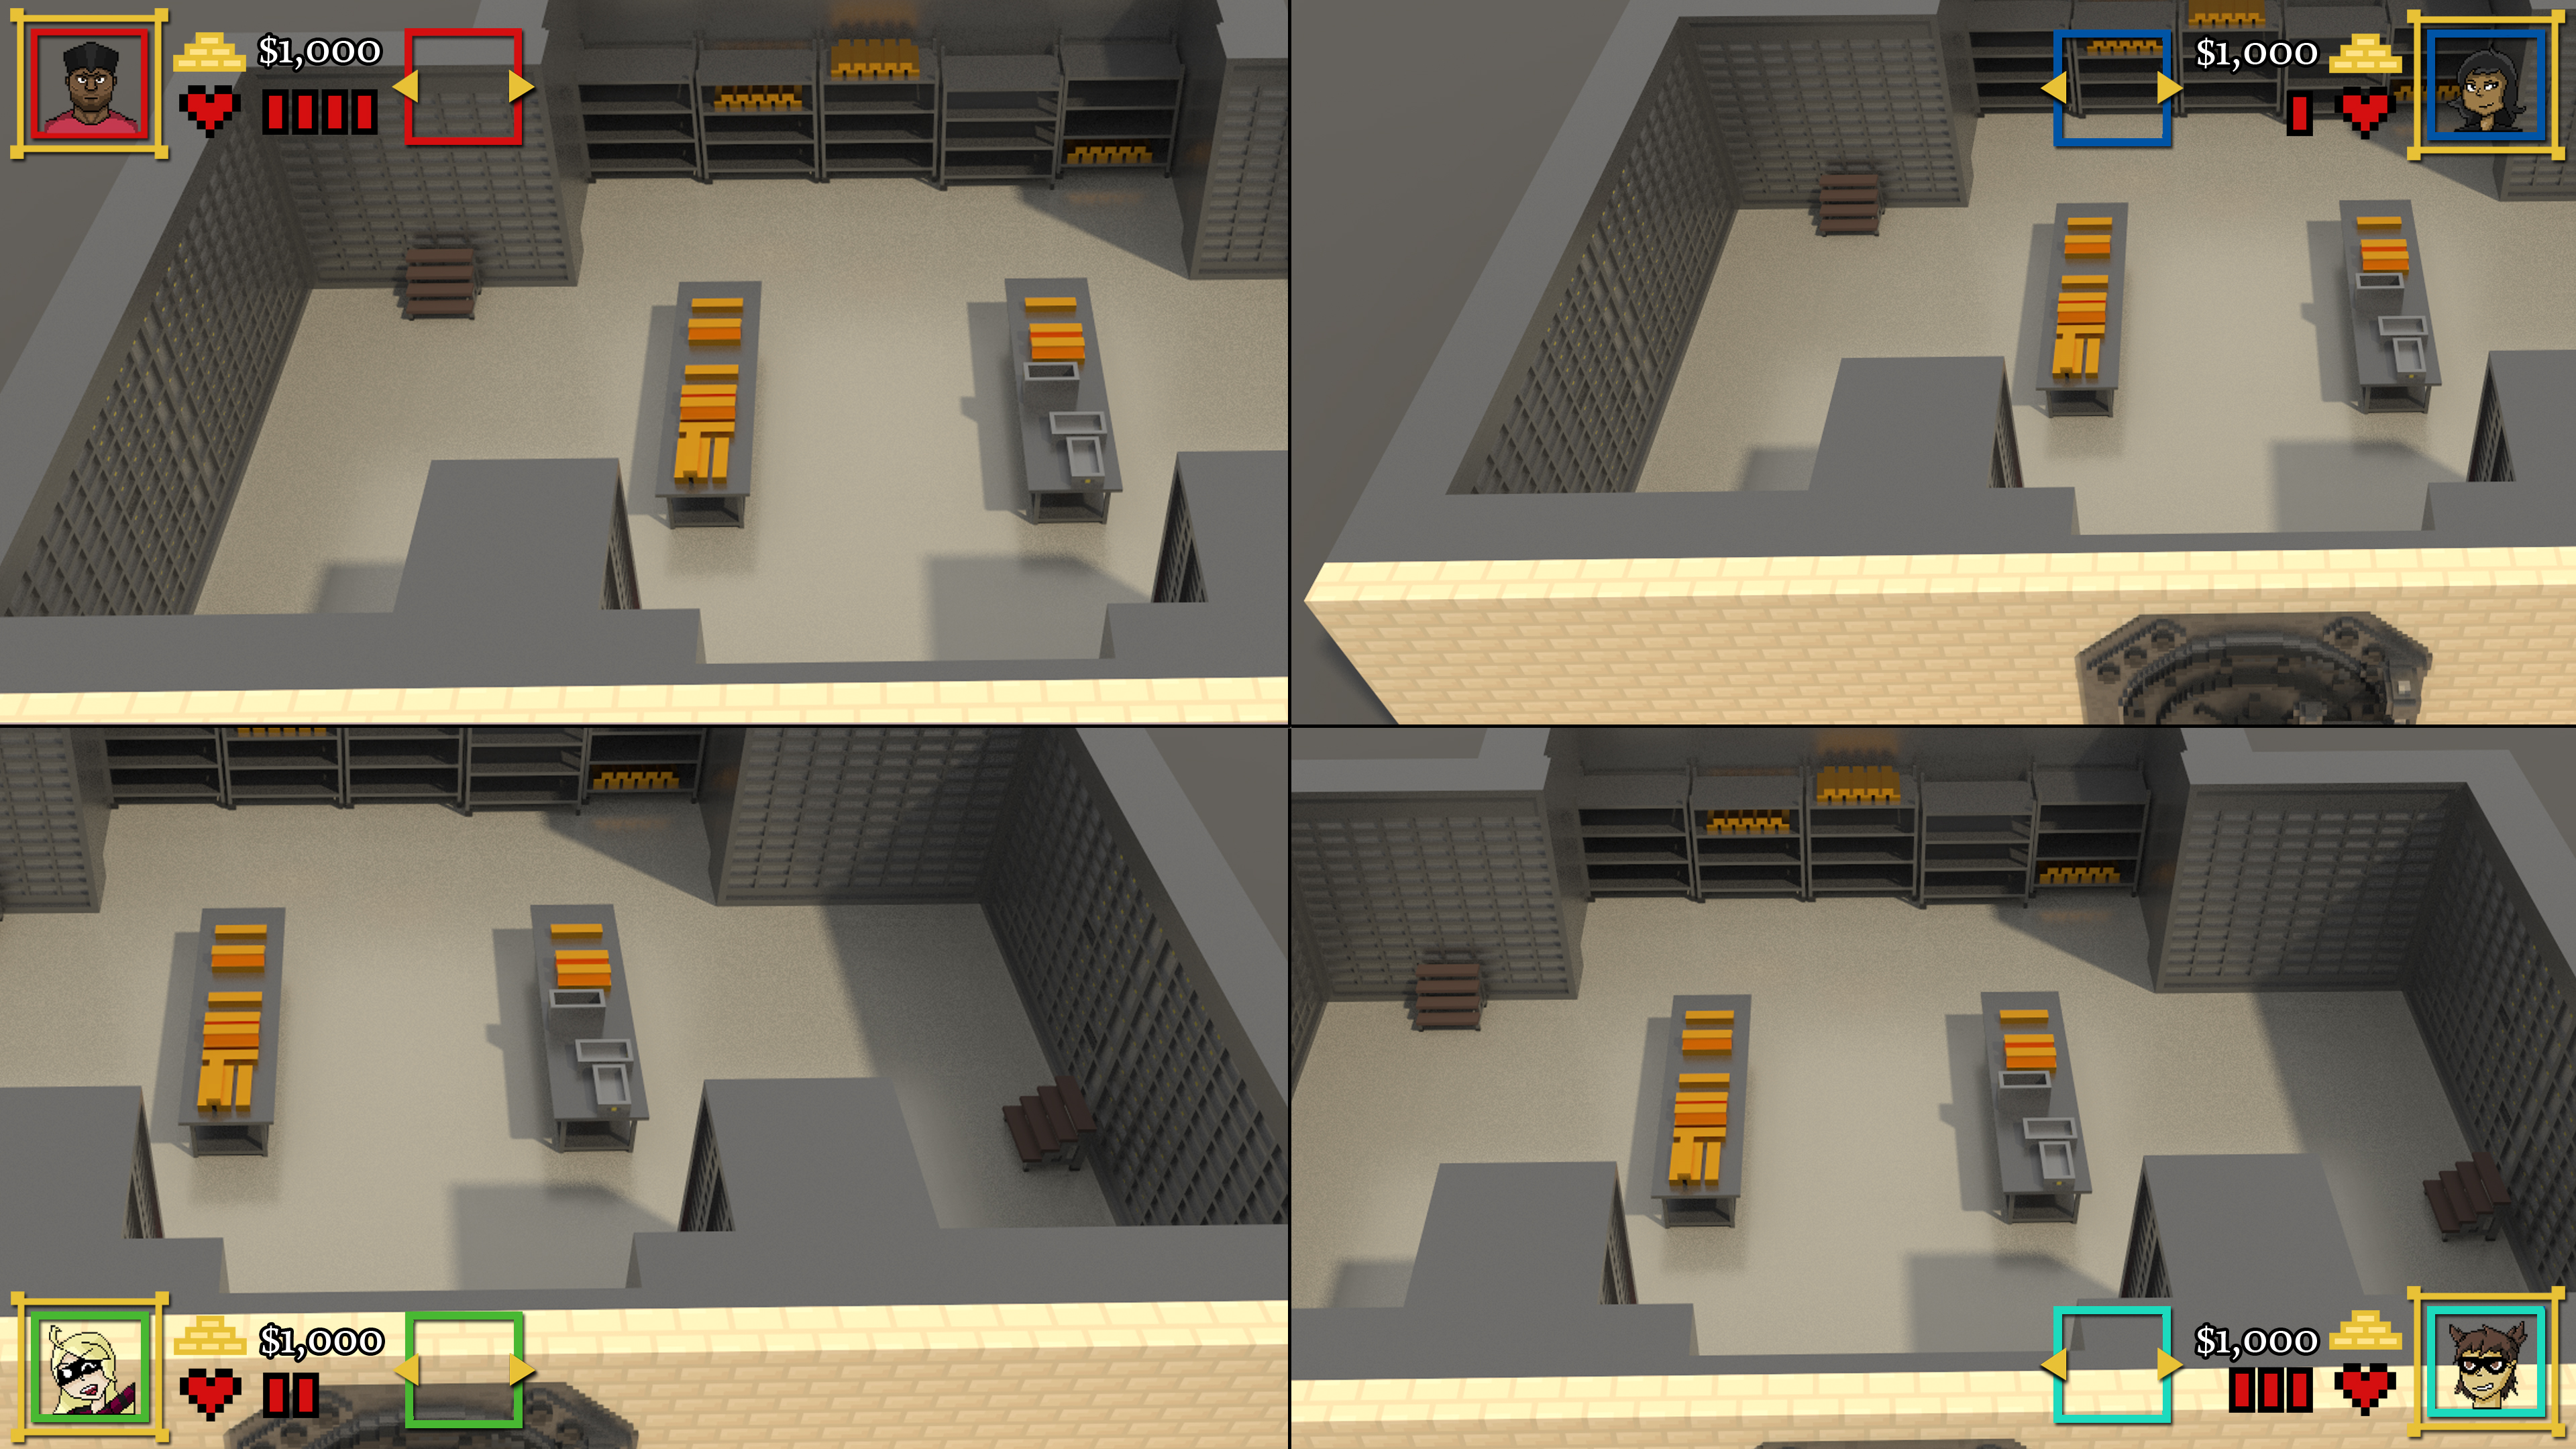
\includegraphics[width=\linewidth]{images/ingameuifinal.jpg}
    \caption{In-game UI}
\end{figure}

\begin{figure}[H]
    \centering
	\includegraphics[width=.4\linewidth]{images/kingui_sarah.jpg}
	
\includegraphics[width=.4\linewidth]{images/shadowui_sarah.jpg}
	
\includegraphics[width=.4\linewidth]{images/jailbirdui_sarah.jpg}
	\includegraphics[width=.4\linewidth]{images/raccoonui_sarah.jpg}
    \caption{Early Character UI}
\end{figure}

\begin{figure}[H]
    \centering
    \begin{subfigure}[b]{0.4\linewidth}
        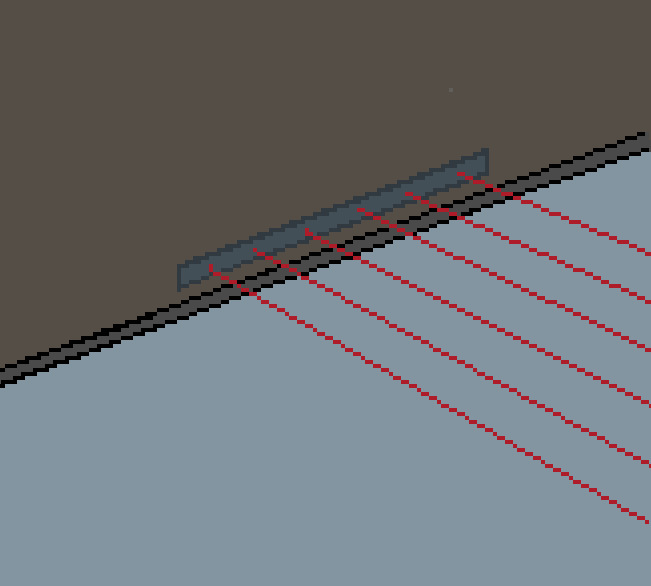
\includegraphics[width=\linewidth]{images/lasertripwire.jpg}
        \caption{Lethal Laser}
    \end{subfigure}
    \begin{subfigure}[b]{0.4\linewidth}
        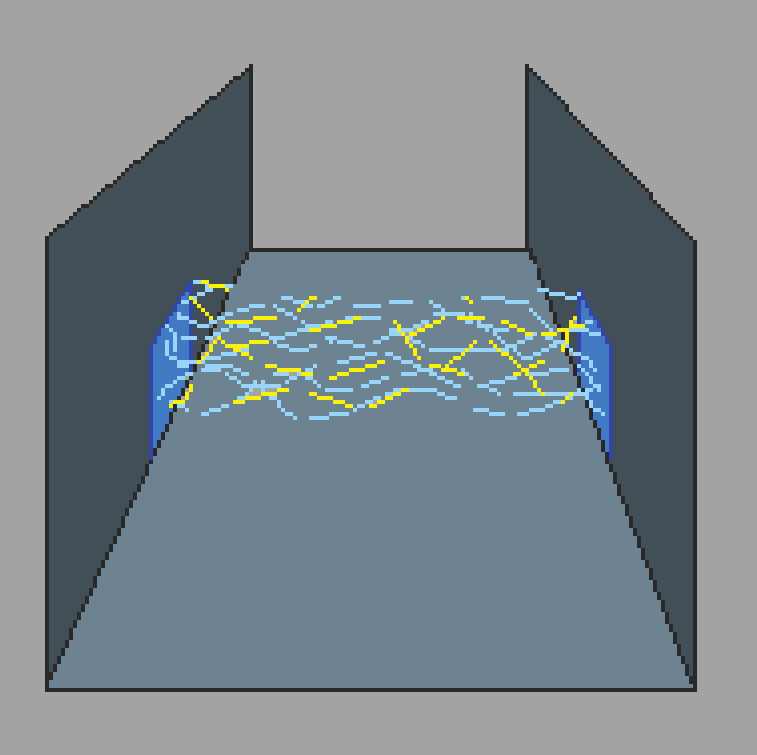
\includegraphics[width=\linewidth]{images/electricfield.jpg}
        \caption{Electric Field}
    \end{subfigure}
    \begin{subfigure}[b]{\linewidth}
        \centering
        
\includegraphics[width=0.4\linewidth]{images/pixil.jpg}
        
\includegraphics[width=0.4\linewidth]{images/camera.jpg}
        \caption{Camera Sensor Early Concept}
    \end{subfigure}
    \caption{Concept of Hazards}
\end{figure}

\begin{figure}[H]
	\includegraphics[width=\linewidth]{images/electricfield1.jpg}
    \caption{Electric Field Concept}
\end{figure}

\begin{figure}[H]
    \centering
	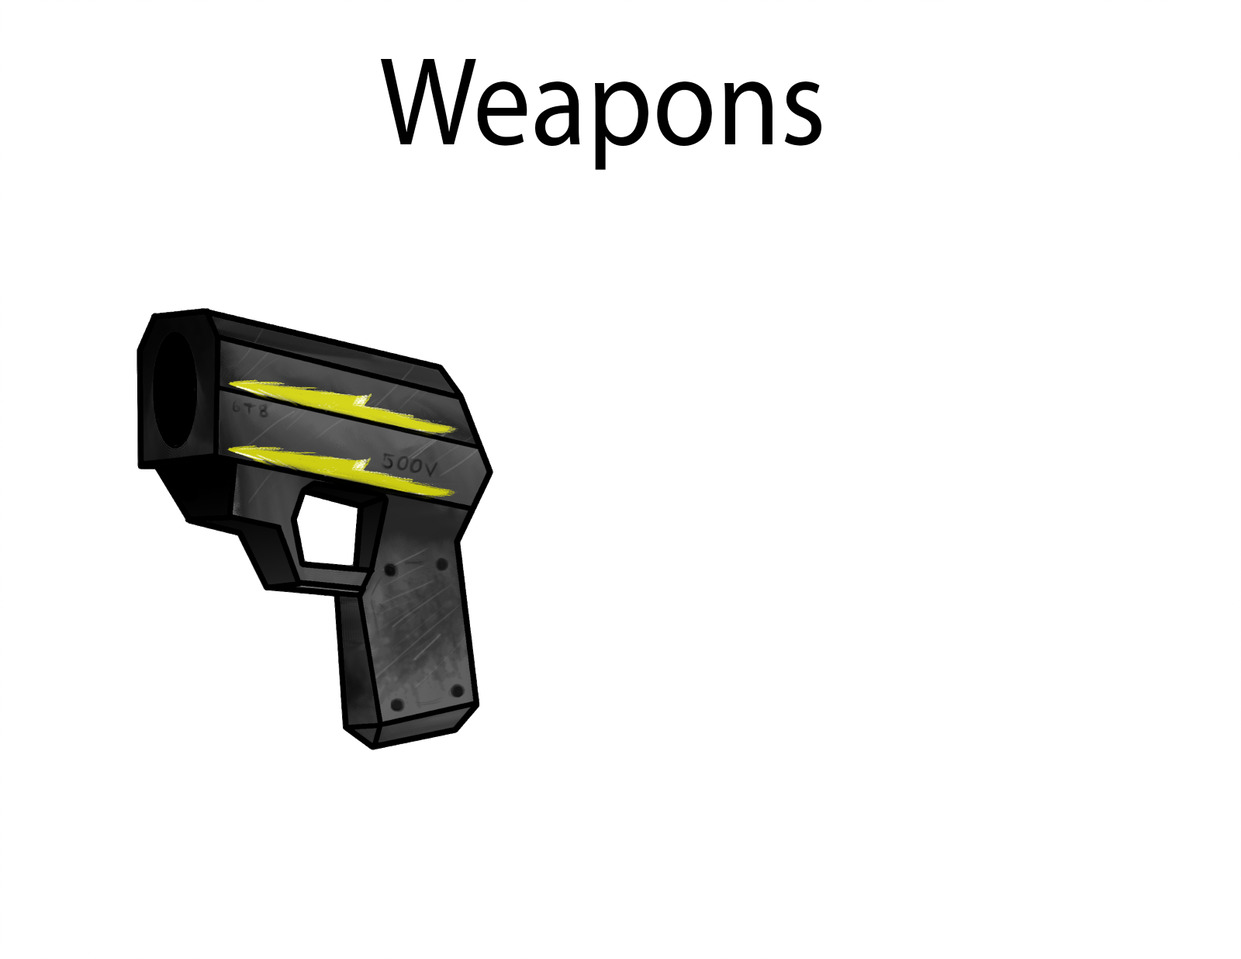
\includegraphics[width=.3\linewidth]{images/taser.jpg}
	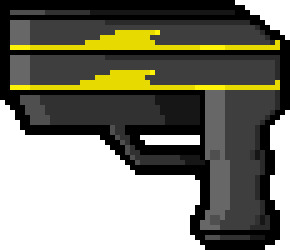
\includegraphics[width=.3\linewidth]{images/zappy_gun.jpg}
	\includegraphics[width=.3\linewidth]{images/zappy_stick.jpg}
    \caption{Stun Gun and Baton Concept Art}
\end{figure}

\begin{figure}[H]
    \centering
	\includegraphics[width=.4\linewidth]{images/drone_face.jpg}
	\includegraphics[width=.4\linewidth]{images/drone_fac2e.jpg}
    \caption{Security Drone}
\end{figure}

\section{Characters}

\begin{figure}[H]
	\includegraphics[width=\linewidth]{images/charactes.jpg}
    \caption{Heist Characters}
\end{figure}

\begin{figure}[H]
    \centering
	\includegraphics[width=.4\linewidth]{images/TheBig.jpg}
	\includegraphics[width=.4\linewidth]{images/TheShadow.jpg}
	\includegraphics[width=.4\linewidth]{images/TheJailbird.jpg}
	\includegraphics[width=.4\linewidth]{images/TheRaccoon.jpg}
    \caption{Individual Heist Character Portraits}
\end{figure}

\section{Environments}

\begin{figure}[H]
    \centering
	\includegraphics[width=.8\linewidth]{images/cinquebank.jpg}
    \caption{Heist Portraits}
\end{figure}

\begin{figure}[H]
    \centering
	\includegraphics[width=.8\linewidth]{images/insidebank.jpg}
    \caption{Heist Portraits}
\end{figure}


\chapter{Appendices}

\section{Asset List}

\subsection{Art}

\subsubsection{Playable Characters}


\begin{tabular}{| p{.45\linewidth} | p{.45\linewidth}|} 
    \hline
    Playable Characters & Description \\ \hline
    Marshal\_`King'  &   Male, athletically built, African American, brown eyes, black hair, primarily long sleeves (top color variations for how many players choose King) dark bottoms and heavy boots/shoes.  \\ \hline
    Olivia\_`Shadow' &   Female, slender built, middle eastern ancestry, brown eyes, black hair, full body catsuit (top color variations for how many players choose King) and knee high black boots.  \\ \hline
    Ana\_`Jailbird'  &   Female, slender, Caucasian, brown eyes, blond hair, wears a mask, and dressed in prison attire from being a consistent escapee.  \\ \hline
    Rocco\_`Racoon'  &   Male, medium built, Caucasian, blue eyes, tattered clothing, hair is disordered with two bunches are pointed up that resembles ears and wears a mask.  \\
    \hline
\end{tabular}

\subsubsection{Non-Playable Characters}

\begin{tabular}{| p{.45\linewidth} | p{.45\linewidth} |}
    \hline    
    Non-Playable Characters &   Description  \\ \hline
    Security\_Drone &    Follows set path to stop players from getting away with gold.  \\ \hline
    A.S.I.A. (Artificial, Security,Intelligence,Administrator) this &   A.S.I.A. controls all of the bank’s security systems that including the drones who will interact with the player through voice lines.  \\
    \hline
\end{tabular}

\subsubsection{Model and Texture List}

\begin{tabular}{| p{.45\linewidth} | p{.45\linewidth} |}
    \hline    
    3D Models   & Description  \\ \hline
    Plants (5)  &   Potted plants to fill the environment \\ \hline
    Filing Cabinets (4) &  Filing Cabinets to fill the environment \\ \hline
    Tables (4)  &  Assorted tables to fill the environment \\ \hline
    King Character  &  King character model \\ \hline
    Jailbird Character  &  Jailbird character model \\ \hline
    Shadow Character    &  Shadow character model \\ \hline
    Racoon Character    &  Racoon character model \\ \hline
    Security Camera &   \\ \hline
    Electric Field  &  Model of electric field hazard + particles \\ \hline
    Lethal Laser    &  Model of laser emitting hazard \\ \hline
    Drone   &  \\ \hline
    Taser   &  \\ \hline
    Baton   &  \\ \hline
    Computers (6)   &  \\ \hline
    Laptops (3) &  \\ \hline
    Papers (3)  &  \\ \hline
    Books (4)   &  \\ \hline
    Couches (3)  &  \\ \hline
    Loveseat    &  \\ \hline
    Desk Chair  &  \\ \hline
    Chairs (4)  &  \\ \hline
    Small Bookshelves (3)   &  \\ \hline
    Large Bookshelves (3)   &  \\ \hline
    Desks (6)   &  \\ \hline
    Teller Windows  &  \\ \hline
    Bank Machine    &  \\ \hline
    Wall Segments(3)    & Assorted styles of wall. (Brick/Plaster/Metal) \\
    \hline
\end{tabular}

\subsubsection{Sprites}

\begin{tabular}{| p{.45\linewidth} | p{.45\linewidth} |}
    \hline 
    Sprites     &   Description  \\ \hline
    Stun\_Sprite     &   Stars spinning around character. Disappears after stun is over.  \\ \hline
    Punch\_Sprite    &   Energy burst from punch animation. Disappears after impact.   \\ \hline
    Stun\_Timer  &   Intuitive circle that hovers above the player’s head to signify how long they are stunned for.   \\ \hline
    Gold\_Channelling\_Sprite   &  \\ \hline
    QuickTimeEvent\_Sprite   &     Displays the sprite object for when the Quick time event happens for players to interact with.  \\ \hline
    Security\_Door\_Lights\_Sprite(optional)   &   Simple triangular sprite that rotates around the alarm lights at the vault to security points.  \\ \hline
    InGame\_Timer\_Sprite(optional)   &   Timer is displayed for when the vault has been infiltrated.   \\ \hline
    LockDown\_Icon\_Sprite    &       \\
    \hline
\end{tabular}

\subsubsection{Animation List}

\begin{tabular}{| p{.45\linewidth} | p{.45\linewidth} |}
    \hline
    Animation List      &   Description     \\ \hline
    King\_Walk\_Animation &   King walks with a heavier gait, lumbering around the bank due to his larger build and being able to carry more gold than other characters.  \\ \hline
    Shadow\_Walk\_Animation   &   Shadow walks with longer and faster gait. Skulking around the bank, with hers swift movements.  \\ \hline
    Jailbird\_Walk\_Animation &   Jailbird walks carefree with looser gait.   \\ \hline
    Raccoon\_Walk\_Animation  &   Raccoon walks with a slight stagger due to his jerky nature.    \\ \hline
    VaultDoor\_Animation &   Vault door opens when player(s) reach the vault and the ‘gear’ spins as a separate object.  \\ \hline
    RoomDoor\_Animation  &   Door to rooms will open when characters enter a room. (physics based when character hits door it moves on a pivot)  \\ \hline
    SecurityDrone\_Attack\_Animation  &   Security drone can engage or retract arm to attack/stun players.    \\ \hline
    SpotLight\_Animation &   Spotlight moves left to right repeatedly.   \\ \hline
    Combat\_Punch    &   All characters have the same general punch animation.   \\ \hline
    Combat\_Weapon\_Shoot     &   All characters have the same general shoot animation. Weapon spawns into character hand.    \\ \hline
    Combat\_Weapon\_BatonSwing    &   All characters have the same general baton hit animation.  Weapon spawns into character hand.   \\ \hline
    Character\_Slow\_Movement     &   Character moves half a speed slower when holding gold.  \\ \hline
    Character\_Menu\_Chosen   &   Character throws fist in air when chosen.   \\ \hline
    Character\_Endgame   &   Character does victory cheer for 1st,2nd,3rd,4th    \\ \hline
    Security\_Drone\_Default  &   Drone moves along the set path normally.    \\ \hline
    Security\_Drone\_Caution  &   Drone moves along the set path slightly faster and LED’s change to orange.  \\ \hline
    Security\_Drone\_HighAlert    &   Drone moves along the set path faster and LED’s change to red.          \\
    \hline
\end{tabular}

\subsubsection{Effects List}

\begin{tabular}{| p{.45\linewidth} | p{.45\linewidth} |}
    \hline
    User-Interface List     &   Description  \\ \hline
    Controls\_UI     &   Display of controller/keyboard to show players the controls of the game.  \\ \hline
    Player\_InGame\_HUD   &   Displays player stats, gold, health, player icon, weapon selected.  \\ \hline
    Menu\_Start\_Screen\_GUI   &   Menu options are displayed (start, characters select,   \\ \hline
    Character\_Selection\_GUI     &   Characters are displayed for players to select between the four characters.   \\ \hline
    Menu\_Pause\_Screen\_GUI   &   Pause options (resume, settings, extras)  \\ \hline
    Player\_Scoreboard\_GUI   &   Displays how many gold that has been obtained to the player throughout/endgame.  \\ \hline
    EndGame\_Victory\_Screen\_GUI  &   Displays the winner with the most gold, second most, third most and lowest at endgame.   \\ \hline
    LowdownTimer\_UI &   Displays timer during lockdown. \\ \hline
    Introduction\_CutScene   &   Comic Book style how the characters get into the bank.  \\
    \hline
\end{tabular}
 
\subsubsection{Cut Scene List}

\subsection{Audio}

\subsubsection{Music}

\begin{tabular}{| p{.45\linewidth} | p{.45\linewidth} |}
    \hline
    Sound & Description \\  \hline
    Infiltration Theme  &     Quiet, tension raising jazz piece, lots of swagger and focus on drums and upright bass \\ \hline
    Scavenging Theme    &     Jazz piece with higher overall volume and faster tempo, high focus on sax lead. \\ \hline
    Lockdown Theme  &     High intensity, fast paced jazz piece. Parts are pure chaos and meant to conflict with each other. Heavy focus on brass. \\ \hline
    Victory Jingle  &     Quick 10 second long sax line, use of positive chordal tones \\ \hline
    Defeat Jingle   &     Quick 10 second long jazz line, negative chordal tones to convey sadness \\
    \hline
\end{tabular}

\subsubsection{Environmental Sounds}

\begin{tabular}{| p{.5\linewidth} | p{.5\linewidth} |}
    \hline
    Sound & Description \\  \hline
    Bank Door Open  &  \\   \hline
    Room Door Open  &  \\   \hline
    Collecting Gold & Cash register “Cha-Ching” \\  \hline
    Losing Gold & Coins dropping \\ \hline
    Electric Field Zap  & Zap \\    \hline
    Lethal Laser Shot   & Laserbeam \\  \hline
    Footsteps   &  \\   \hline
    Lockdown Siren  & Loud Naval siren \\   \hline
    Drones Ambient patrol   & Machine whirring \\   \hline
    Drones Pursuit  & Machines aggressively beeping \\  \hline
    Drones Attacking    & Loud zap sounds \\    \hline
    Set Trap    & Click \\  \hline
    Pick up Trap    & Click \\
    \hline
\end{tabular}


\subsubsection{Weapon Sounds}

\begin{tabular}{| p{.45\linewidth} | p{.45\linewidth} |}
    \hline
    Sound & Description \\  \hline
    Stun Gun Pickup     & Click \\ \hline
    Stun Gun Fire   & Muzzled gunshot \\ \hline
    Stun Gun Hit    & Zap \\ \hline
    Stun Gun Out of Ammo    & Gun firing empty clip \\ \hline
    Electric Baton Pickup   & Click \\ \hline
    Electric Baton Fire     & Swinging bat through air \\ \hline
    Electric Baton Hit  & Whack and zap \\ \hline
    Electric Baton Out of Time  & Open electric current powering down \\ \hline
    Basic Melee Weapon Hit  & Whack \\
    \hline
\end{tabular}

\subsubsection{Interface Sounds}

\begin{tabular}{| p{.45\linewidth} | p{.45\linewidth} |}
    \hline
    Sound & Description \\  \hline
    Quicktime Event Success &     Electric device being powered down \\ \hline
    Quicktime Event Fail    &     Quiet alarm beeping \\ \hline
    Open Menu   &     Vault opening \\    
    \hline
\end{tabular}

\subsubsection{Voice}

\begin{tabular}{| p{.45\linewidth} | p{.45\linewidth} |}
    \hline
    Sound & Description \\  \hline
    Enter Bank(4)   &   \\ \hline
    Exit Bank(4)    &   \\ \hline
    Pick up Trap(4) &   \\ \hline
    Pick up Weapon(4)   &   \\ \hline
    Spot Security Drone(4)  &   \\ \hline
    Taking Damage(4)    &   \\ \hline
    Collecting Gold(4)  &   \\ \hline
    Losing Gold(4)  &   \\ \hline
    Taunt(4)    &   \\ \hline
    Joke(4) &   \\ \hline
    Victory(4)  &   \\ \hline
    Defeat(4)   &   \\ \hline
    Capture(4)  &   \\
    \hline
\end{tabular}

\end{document}
